\section{Analýza problému}
V súčasnej dobe patrí platforma Arduino medzi populárne elektronické platformy na svete. Jeho výhodou je otvorený zdrojový kód, jednoduchosť použitia ale aj možnosť vytvárať komplexnejšie projekty. Vďaka týmto spomenutým aspektom Arduino je využívané úplnými začiatočníkmi, ale aj prokročilejšími používateľmi \cite{WhatArduinoArduino}.
 Práve pri komplexnejších projektoch sa často môžeme stretnúť časovo kritickými 
 úlohami, ako aj s nutnosťou zastaviť aktuálne vykonávaný kód a reagovať na externý vstup. To pri štandardnom sekvenčnom písaní kódu nemusí byť jednoduché a často to môže končiť kódom, ktorý je len veľmi ťažko udržiavateľný. Preto sa na to pri tomto type programovania využíva udalosťami riadená paradigma. Táto paradigma môže byť ďalej modelovaná napríklad pomocou Petriho sieti \cite{bastidePetriNetBased1995}, alebo aj za pomoci konečných stavových automatov \cite{dashEventDrivenProgramming2011}.
 TODO: DOKONCIT 

\section{Prerušenia}
\noindent Vo vstavaných systémoch prerušenie upozorní procesor na udalosť, ktorá nastala a je potrebné, aby jej procesor venoval pozornosť. Často ide o signály vygenerované perifériami procesora. Procesor na prerušenie zareaguje pozastavením vykonávania aktuálnej aktivity, uložením jej stavu a začatím vykonávania kódu na inej pamäťovej adrese \cite{wangAutomaticDetectionValidation2017}. \par 
Táto adresa je definovaná v takzvanom \textit{vektore prerušení} (interrupt vector). \textit{Vektor prerušení} je konfiguravateľné alebo pevne dané miesto v pamäti, ktoré špecifikuje adresu, kde má procesor pokračovať vo vykonávaní kódu. Každé podporované prerušenie sa musí nachádzať v tomto vektore. Blok pamäte kam odkazuje vektor prerušení, sa nazýva \textit{obsluha prerušenia}. V anglickej literatúre sa používa výraz \textit{interrupt service routine} \textit{(ISR)}, preto aj my budeme ďalej používať skratku  ISR. Po vykonaní  ISR sa procesor vráti k predtým vykonávanej aktivite. \par
\textit{Radič prerušení} je periférne zariadenie, ktoré spravuje prerušenia pre procesor. Niektoré architektúry procesorov majú integrovaný sofistikovaný radič prerušení (napríklad AVR alebo MSP430), zatiaľ čo iné obsahujú iba základný ovládač, ktorý si vyžaduje ďalší externý radič prerušení (napríklad ARM alebo x86). \par
Prerušenie je v stave \textit{čakania}, ak daná udalosť nastala a radič prerušení dané prerušenie zaregistroval, avšak ešte sa nezačalo vykonávanie ISR.  O \textit{zmeškanom prerušení} hovoríme, keď udalosť prerušenia nastala, ale radič prerušení sa o tom nedozvedel. Toto väčšinov nastáva v situácii, keď je prerušenie v stave čakania a udalosť nastane znova. \par
Prerušenie je \textit{zakázané}, keď je na hardvérovej úrovni zabránené spusteniu prerušenia. Vo všeobecnosti, väčšina prerušení má svoj dedikovaný bit v hardvérových registroch, ktorý povoľuje, respektíve zakazuje vykonanie prerušenia. Na väčšine procesorov je taktiež možné vypnúť všetky prerušenia vynulovaním bitu, ktorý globálne zakazuje/povoľuje prerušenia. Tento bit sa nazýva aj \textit{master interrupt enable bit}.\par 
Prerušenie nastane pri splnení nasledujúcich podmienok:
\begin{enumerate}
    \item Master interrupt enable bit je nastavený.
    \item Dedikovaný bit prerušenia je nastavený.
    \item Prerušenie je v stave čakania.
    \item Procesor sa nachádza v stave medzi vykonaním dvoch inštrukcií alebo vykonáva inštrukciu, ktorú je možné prerušiť.
    \item Nenastalo žiadne prerušenie, ktoré splnilo podmienky 1-4 a má vyššiu prioritu.
\end{enumerate} \par

\textit{Latencia} prerušenia je časový interval od momentu kedy boli splnené podmienky vykonania prerušenia až po chvíľu začatia vykonávania ISR daného prerušenia. Ak sa objaví ďalšie prerušenie s vyššou prioritou, latencia prerušenia s nižšou prioritou môže byť veľká. K dĺžke latencie prispievajú aj vyššie spomínané podmienky vykonania prerušenia, keďže kontrola či sú bity nastavené alebo dokončenie vykonávania aktuálnej inštrukcie procesorom trvá nejaký čas. \par
Veľká väčšina procesorov podporuje aj prerušenia, ktoré nie je môžné vypnúť (non-maskable interrupt - NMI). Používajú sa v prípade nastania fatálnych chýb z, ktorých nie je možné žiadnym spôsobom vykonať nápravu programu
\cite{regehrSafeStructuredUse2007}. \par
Prerušenia je možné vnímať aj ako udalosti. Pri ich využívaní v programe je preto možné hovoriť o programovaní pomocou udalosťami riadenej paradigmy. Takýto program je možné označiť ako \begin{math}P=Task || ISR\end{math}, kde \begin{math}Task\end{math} je hlavný program pozostávajúci z jednej alebo viacerých úloh (vlákien) a  \begin{math}ISR\end{math} kde \begin{math}ISR=ISR_1||ISR_2||ISR_3||..||ISR_N\end{math} sú obsluhy prerušení.
Indexy daných \begin{math}ISR\end{math} predstavujú číslo prerušenia. Čím je číslo väčšie, tým menšiu prioritu dané prerušenie má \cite{wangAutomaticDetectionValidation2017}. \par Prerušenia sú väčšinovo využívané na indikovanie dvoch typov udalostí. Prvou je udalosť vykonaná používateľom, kde patrí napríklad stlačenie tlačidla. Druhou je prijatie dát z periferného zariadenia. Ako príklad môžeme uviesť UART protokol \cite{wangAutomaticDetectionValidation2017}.
\section{Konečný stavový automat}
\noindent Existuje množstvo spôsobov ako modelovať správanie sytémov. Jedným z 
najstarších a najznámejších je modelovanie pomocou konečného stavového automatu.
Vďaka takejto abtrakcii môžeme o problémoch rozmýšľať ako o stavoch, ktoré nastali v určitom čase a charakterizujú to ako sa systém má správať. 
Táto technika však nie je limitovaná len na modelovanie softvérových systémov. Využíva sa aj v iných oblastiach ako napríklad vo fyzike a biológii \cite{WaybackMachine2014}. 
\par Častou úlohou vstavaných systémov je reagovanie na udalosti, ktoré nastali  na rôznych 
periférnych zariadeniach. To o akú reakciu pôjde záleží od dvoch faktorov. Prvým je typ
udalosti, ktorá nastala. Druhým je kontext v akom udalosť nastala 
(napríklad sekvencia minulých udalostí). Stavový automat robí obsluhu udalostí explicitne závislými od povahy udalosti a od kontextu (stavu) systému. 
Stav veľmi efektívne zachytáva relevantné aspekty histórie systému. 
Stav môže abstrahovať všetky možné (relevantné ale i irelevantné) sekvencie udalostí a zachytiť len tie podstatné \cite{samekStateMachinesEventDriven2016}.
\par Konečný stavový automat je výpočtový model, ktorý sa používa na simuláciu sekvenčnej logiky. 
Poznáme dva typy konečných stavových strojov: deterministický konečný automat (DKA)  a nedeterministický stavový automat (NKA) \cite{FiniteStateMachines}. 

\subsection{Deterministický konečný automat}
\noindent Deterministický konečný automat $\mathcal{M}$ je definovaný päticou ($\Sigma$ ,$\mathcal{Q}$ , $q_0$, $\mathcal{F}$, $\delta$), kde
\begin{itemize}
    \item $\Sigma$ je neprázdna a konečná vstupná abeceda $\mathcal{M}$
    \item $\mathcal{Q}$ je konečná množina stavov $\mathcal{M}$
    \item $q_0$ je počiatočný stav $\mathcal{M}$
    \item $\mathcal{F}$ $\subseteq$ $\mathcal{Q}$ je množina konečných stavov $\mathcal{M}$
    \item $\delta$ je prechodová funkcia  \begin{math}\delta : Q \times \Sigma \Rightarrow Q\end{math}
\end{itemize}

Automat musí definovať presne jednu prechodovú funkciu pre každý symbol v $\Sigma$ pre každý stav v $\mathcal{Q}$ \cite{FiniteStateMachines}.
 DKA môže byť reprenzentovaný pomocou diagramu, ktorý vidíme na obrázku č.\ref{figure:dfa1}.

\newpage

\begin{figure}[!h]
    \centering
    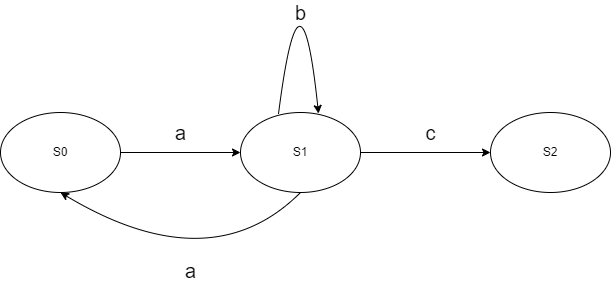
\includegraphics[width=0.70\textwidth]{img/dfa.png}
    \caption{Príklad deterministického konečného stavového automatu}
    \label{figure:dfa1}
\end{figure}

Rovnaký DKA môže byť popísaný aj nasledovne:
Nech $\mathcal{M}$ je pätica ($\Sigma$ ,$\mathcal{Q}$ , $q_0$, $\mathcal{F}$, $\delta$) kde, 

\begin{itemize}
    \item \begin{math} \Sigma = \{a, b ,c \}  \end{math}
    \item \begin{math} Q = \{S0, S1, S2 \}  \end{math}
    \item \begin{math} q_0 = \{S0 \}  \end{math}
    \item $\mathcal{F}$ \begin{math} = \{S2\}  \end{math}
\end{itemize}
a prechodová funkcia $\delta$ je daná tabuľkou číslo \ref{table:dfaPrechodovaFunckcia}:

\begin{table}[!htbp]    
    \begin{center}
    \begin{tabular}{c c|c}
    $\mathcal{Q}$ & $\Sigma$ & $\Rightarrow$ $\mathcal{Q}$  \\ \hline
    S0 & a & S1 \\ 
    S0 & b & S0 \\ 
    S0 & c & S0 \\ 
    S1 & a & S0 \\
    S1 & b & S1 \\  
    S1 & c & S2 \\  
    \end{tabular}
    \caption{Prechodová funkcia automatu $\mathcal{M}$}
    \label{table:dfaPrechodovaFunckcia}
    \end{center}
    \end{table}


\subsection{Nedeterministický konečný automat}
\noindent Podobne ako DKA aj NKA je reprenzentovaný ako  pätica ($\Sigma$ ,$\mathcal{Q}$ , $q_0$, $\mathcal{F}$, $\delta$) kde
\begin{itemize}
    \item $\Sigma$ je neprázdna a konečná vstupná abeceda $\mathcal{M}$
    \item $\mathcal{Q}$ je konečná množina stavov $\mathcal{M}$
    \item $q_0$ je počiatočný stav $\mathcal{M}$
    \item $\mathcal{F}$ $\subseteq$ $\mathcal{Q}$ je množina konečných stavov $\mathcal{M}$
    \item $\delta$ je prechodová funkcia  \begin{math}\delta : Q \times \Sigma \Rightarrow Q\end{math}
\end{itemize}

Narozdiel od DKA, NKA nevyžaduje definíciou prechodovej funkcie pre každý symbol 
patriaci $\Sigma$. Zároveň v NKA môže byť definovaná viac ako jedna prechodová funkcia $\delta$ pre symbol z $\Sigma$. 
Taktiež je možné použiť aj takzvané nulové prechody. 
Tie sa označujú ako $\epsilon$ a dovoľujú prechod z jedného stavu do druhého bez potreby prečítania akéhokoľvek symbolu patriaceho $\Sigma$ \cite{FiniteStateMachines}.
\section{Programovacie paradigmy}
\noindent Programovacia paradigma je spôsob riešenia programátorských problémov \cite{Samuel2018AnII}. Poznáme veľké množstvo programovacích paradigiem. Medzi ne patria aj nasledujúce štyri:
\begin{itemize}
  \item Imperatívna paradigma.
  \item Funkcionálna paradigma.
  \item Objektovo orientovaná paradigma.
  \item Udalosťami riadená paradigma.
\end{itemize}

\subsection{Imperatívna paradigma}
\noindent Základnou myšlienkou je príkaz, ktorý má merateľný dopad na aktuálny stav 
programu. Pri imperatívnej paradigme je rovnako dôležité aj poradie príkazov. Stav 
programu po vykonaní príkazov v ľubovoľnom poradí nemusí byť rovnaký ak by boli príkazy 
vykonané v inom poradí \cite{imperativParadigm}. 

\subsection{Funkcionálna paradigma}
\noindent Je postavená na koncepte matematických funkcií, ktoré používajú podmienené 
výrazy a rekurziu na vykonanie výpočtu. Zameriava sa na výsledok, nie na spôsobom akým 
sa k výsledku dopracovať. Jednou z jeho základných vlastností je nemennosť dát. To 
znamená, že ak už bola nejaká štruktúra vytvorená nie je možné meniť jej vnútorný stav. 
V prípade potreby zmeny stavu je nutné celú štruktúru vytvoriť odznova. Medzi 
najpoužívanejšie funkcionálne jazyky patrí Haskell, Clojure alebo SQL \cite{functionalParadigm}.

\subsection{Objektovo orientovaná paradigma}
\noindent Paradigma, ktorej myšlienka je inšpirovaná svetom okolo nás. Čokoľvek môže 
byť objekt. Auto, dom, kniha či dokument. Každý z týchto objektov má špecifické vlastnosti 
a určité správanie. Rovnakým spôsobom modelujeme program. Takéto rozmýšľanie o 
objektoch nám umožňuje písať kód, ktorý je jednoduchší na pochopenie a zároveň je 
vďaka tomu možné kód rozdeliť na menšie časti. Tieto časti kódu sú následne 
jednoduchšie udržiavateľné. Medzi hlavné princípy objektovo orientovaného prístupu 
patrí dedičnosť, zapuzdrenosť, polymorfizmus a abstrakcia \cite{objectOrientedParadigm}
. Populárne programovacie jazyky podporujúce túto paradigmu sú Python, C\# a Java \cite
{stack-overflow-survey-2020}.

\subsection{Udalosťami riadená paradigma}
\noindent V tejto paradigme je tok programu určený udalosťami. Udalosti môžu byť
rôzne. Väčšinou sa generujú pri akciách používateľa ako napríklad stlačenie tlačidla
alebo písanie na klávesnici. Udalosti môžu byť generované aj rôznymi perifériami systému ako napríklad pomocou senzorov alebo komunikačnými protokolmi. Niekedy môže byť udalosť generovaná interne, napríklad časovačom alebo prerušením. Bez ohľadu na
zdroj alebo typ udalostí, udalosťami riadené programovanie 
hovorí o programovacej paradigme, v ktorej sa tok
programu určujuje udalosťami.
\par V dnešnej dobe je možné použiť akýkoľvek programovací jazyk na implementáciu tejto paradigmy. Implementácia by mala zahrňovať nasledujúce časti:
\begin{enumerate}
  \item Zachytávanie udalostí
\end{enumerate}

\noindent \par 
Táto časť programu je zodpovedná za zachytávanie vygenerovaných udalostí, ich identifikáciu a prípadné predspracovanie udalosti.

\begin{enumerate}[resume]
  \item Rozposielanie udalostí
\end{enumerate}

\noindent \par
Po zachytení udalosti nasleduje jej rozposlanie. V tejto časti program identifikuje obsluhy udalostí, ktoré je potrebné vyvolať na základe typu udalosti. Ak daný typ udalosti nemá zaregistrovanú žiadnu oblužnú funkciu, program buď udalosť odignoruje, alebo vygeneruje výnimku.

\begin{enumerate}[resume]
  \item Obsluha udalostí
\end{enumerate}
 
\noindent \par
Časť programu, ktorá je zodpovedná za konečnú obsluhu udalosti. Tu sa nachádza kód, ktorý vykonáva potrebnú funkcionalitu. Ako príklad môžeme uviesť stlačenie tlačidla na klávesnici v textovom editore. Po stlačení sa práve tu nachádza logika programu, ktorá zabezpečí vykreslenie písmena na obrazovku.

\begin{figure}[!htbp]
  \centering
  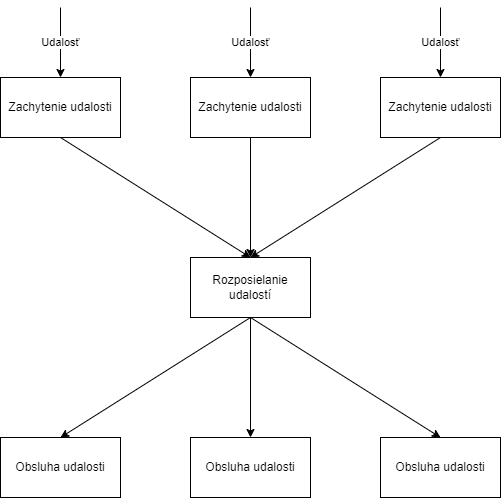
\includegraphics[width=0.60\textwidth]{img/event-driven-schema.png}
  \source{\cite{dashEventDrivenProgramming2011}}
  \caption{Schéma implementácie udalosťami riadeného programovania}
  \label{figure:event-driven-schema}
\end{figure}

\par
Udalosťami riadené programy je možné rozdeliť na dva typy. Prvým typom sú programy, ktoré si neuchovávajú aktuálny stav v ktorom sa nachádzajú. To znamená, že pri obluhe udalosti vykonajú vždy rovnakú aktivitu bez ohľadu na to aké udalosti nastali v minulosti. Druhým typom sú programy, kde tok vykonávania závisí nielen od aktuálnej udalosti, ale aj sledu predchádzajúcich udalostí \cite{dashEventDrivenProgramming2011}. 
\par Táto diplomová práca sa venuje práve týmto druhým typom udalosťami riadených programov a ich modelovaním pomocou deterministických konečných automatov.

\section{Ukážka glossaries}
\noindent Verzia FEIstyle 1.5 používa glossary\footnote{\url{https://www.ctan.org/pkg/glossaries?lang=en}} balík.
\acrfull{cdma} je dlhá skratka naopak \acrshort{gsm} je skratka v krátkej forme.
\section{Recitácia}
Citujem všetky zdroje v \textbf{bibliography.bib}, \cite{t00}. \newline Good luck.
\section{Možnosti anonymizácie}
\noindent Anonymizácia znamená zmena alebo úprava údajov tak, aby sa podľa nich nedala jednoznačne určiť osoba, ktorej tieto údaje patria \cite{t01}. Existuje niekoľko spôsobov, ktorými môžeme dosiahnuť rôznu úroveň anonymizácie na internete: od mazania cookies súborov po ukončení prehliadania webových stránok až po používanie operačných systémov, ktoré sú na anonymite založené; od bezplatných možností až po komerčné verzie.  
\newline Nasleduje priblíženie niektorých možnosti anonymizácie.

\subsection{Súkromné prehliadanie}
\noindent Najpoužívanejšie internetové prehliadače súčasnosti majú v sebe zabudovanú funkcionalitu, ktorá dokáže čiastočne anonymizovať prístup na internet. Táto funkcionalita blokuje ukladanie navštívených stránok do histórie a nezaznamenáva súbory, ktoré sa stiahnu z~internetu. \acrshort{sw} a \acrlong{hw} sú skratky.

\begin{table}[!htbp]
\caption{Moduly a ich funkcie pri anonymizácii}
\label{modulyVlastnosti}
\begin{center}
\begin{tabular}{p{4cm}|c|c|c|c|c|c|c|c|c|c|c|c|c|c|c}
& \multicolumn{14}{c}%
	 {\textbf{Funkcia}}\\ \hline
&&&& & &\multicolumn{8}{c}%
	 {Modifikácia}\\ 
\textbf{Modul} &\begin{sideways} zobrazenie hlavičky \end{sideways} &\begin{sideways} blokovanie skriptov \end{sideways} &\begin{sideways} zmena IP \end{sideways} & \begin{sideways} zmena lokalizácie \end{sideways} & \begin{sideways} zmazanie/blokovanie cookies \end{sideways} & \begin{sideways} blokovanie trackerov \end{sideways}  & \begin{sideways} popis \end{sideways} & \begin{sideways}používateľský agent\end{sideways} & \begin{sideways} kódové označenie prehliadača \end{sideways} & \begin{sideways} názov prehliadača \end{sideways} & \begin{sideways} verzia prehliadača \end{sideways} & \begin{sideways} platforma \end{sideways} & \begin{sideways} výrobca prehliadača \end{sideways} & \begin{sideways} označenie výrobcu prehliadača \end{sideways} \\ \hline
User agent switcher & & & & & &  & X & X & X & X & X & X & X & X  \\ \hline
Ghostery &  && & & X & X &  &  & & & & & & \\  \hline
Better privacy && &  & & X &  &  &  & & & & & & \\  \hline
Anonymox &  && X & X & X &  & X & X & & & & & & \\  \hline
Modify headers & & &  &  & X &  &  & X &  &  &  & & &  \\  \hline
Request policy & & &  &  & & X  &  &  &  &  &  & & &   \\  \hline
Live HTTP headers & X& &  &  & &  &  &  &  &  &  & & &   \\  \hline
User agent awitcher & & &  &  & &  & X & X &  &  &  & & &   \\  \hline
Header hacker & & &  &  & &  & X & X & X & X & X & X & X & X    \\  \hline
Mod header & & &  &  & &  & X & X & X & X & X & X & X & X    \\  \hline
Script no & &X &  &  & &  &  &  &  &  &  &  &  &     \\  \hline
No script & &X &  &  & &  &  &  &  &  &  &  &  &     \\  \hline
Proxify it & & &X  & X & &  &  &  &  &  &  &  &  &     \\  \hline
I'm not here & & &  & X & &  &  &  &  &  &  &  &  &     \\  \hline
Get edition & &X &X &X &X&X &  &  &  &  &  &  &  &     \\  \hline
Anonymous browsing toolbar & & & X & X & &  &  &  &  &  &  &  &  &     \\  \hline
Easy hide your IP and surf & & & X & X& &  &  & X & X & X & X &  &  &     \\  \hline
\end{tabular}
\end{center}
\end{table}

\subsection{Anonymná sieť}
\noindent Anonymná sieť je sieť serverov, medzi ktorými dáta prechádzajú šifrované. V anonymných sieťach dáta prechádzajú z počítača používateľa, odkiaľ bola požiadavka poslaná, cez viaceré proxy smerovače, z ktorých každý správu doplní o smerovanie a zašifruje vlastným kľúčom. Cesta od ...


\subsection{Funkcionalita}
\noindent  Rozšírenie tiež okrem splnenia špecifikácie malo pre prehľadnosť a overenie funkčnosti zobrazovať údaje, ktoré boli na server odoslané. Zoznam údajov odoslaných na server, sa mal ukladať do krátkodobej histórie, aby nemal používateľ k dispozícií len najnovšie údaje, ale aj údaje odoslané v nejakom časovom období. Nejaky listing z priloh \ref{lst:sublime}.

\subsubsection{Funkcionalita2}
\noindent Samozrejmosťou bolo nastavenie zapnutia rozšírenia pri štarte, prípadne interval zmeny odosielaných údajov.

\subsection{Vzhľad}
\noindent Dôležitou požiadavkou kladenou na rozšírenie bolo príjemné používateľské rozhranie. Z~tohto dôvodu malo rozšírenie obsahovať zoznam modifikovaných vlastností a tlačidlo pre prístup k nastaveniam rozšírenia v jednoduchej a praktickej forme. Predpokladaný vzhľad je zobrazený na obrázku č. \ref{vzhladobr}.
\begin{figure}[!htbp]
  \centering
  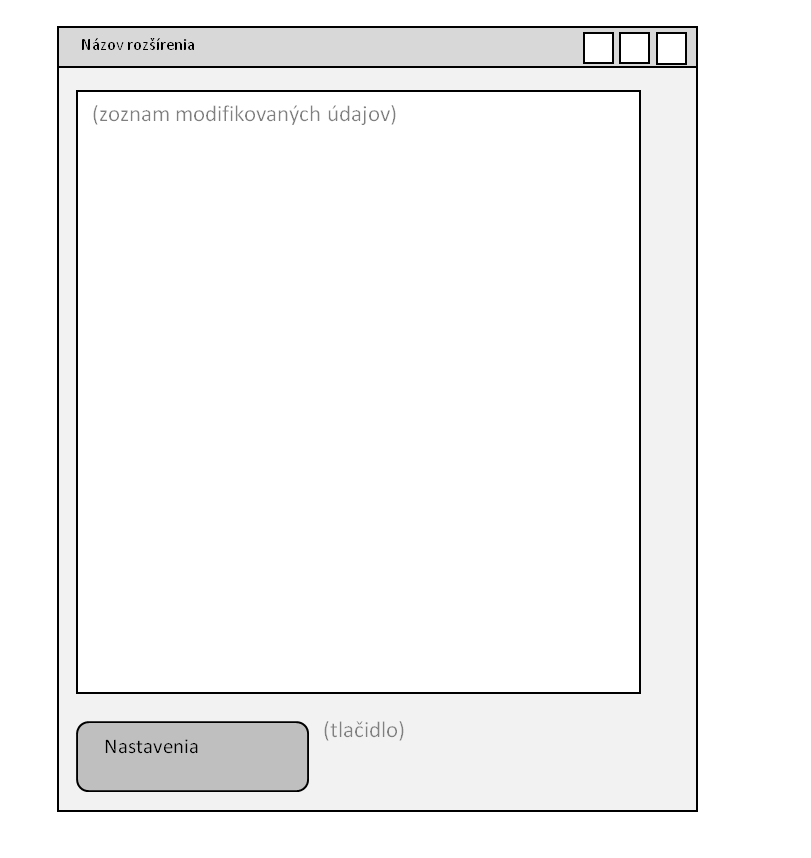
\includegraphics[width=8cm]{img/vzhlad.png}
  \caption{Predpokladaný vzhľad rozšírenia.}
  \label{vzhladobr}
\end{figure}	 
\noindent Dôležitou požiadavkou kladenou na rozšírenie bolo príjemné používateľské rozhranie.\cite{t00} Z~tohto dôvodu malo rozšírenie obsahovať zoznam modifikovaných vlastností a tlačidlo pre prístup k nastaveniam rozšírenia v jednoduchej a praktickej forme. Predpokladaný vzhľad je zobrazený na obrázku č. \ref{vzhladobr}.

\begin{algorithm}
\scriptsize
\begin{algorithmic}
 \STATE <text>
 \IF{<condition>} \STATE {<text>} \ELSE \STATE{<text>} \ENDIF
 \IF{<condition>} \STATE {<text>} \ELSIF{<condition>} \STATE{<text>} \ENDIF
 \FOR{<condition>} \STATE {<text>} \ENDFOR
 \FOR{<condition> \TO <condition> } \STATE {<text>} \ENDFOR
 \FORALL{<condition>} \STATE{<text>} \ENDFOR
 \WHILE{<condition>} \STATE{<text>} \ENDWHILE
 \REPEAT \STATE{<text>} \UNTIL{<condition>}
 \LOOP \STATE{<text>} \ENDLOOP
 \REQUIRE <text>
 \ENSURE <text>
 \RETURN <text>
 \PRINT <text>
 \COMMENT{<text>}
 \AND, \OR, \XOR, \NOT, \TO, \TRUE, \FALSE
\end{algorithmic}
\caption{Ukážka príkazov pre algorithmic}  
\label{alg:preview}  
\end{algorithm}

\begin{lstlisting}[
  caption={Ukážka algoritmu},
  label={lst:main-c},
  language=c
]
/* Hello World program */

#include<stdio.h>

struct cpu_info {
    long unsigned utime, ntime, stime, itime;
    long unsigned iowtime, irqtime, sirqtime;
};

main()
{
    printf("Hello World");
}
\end{lstlisting}
